\section{Amplificatore invertente e non-invertente}

\begin{figure}[h!]
\centering
		\begin{minipage}[c]{.4\textwidth}
			\centering

			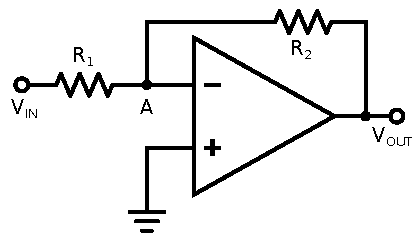
\includegraphics[width=.65\textwidth]{ccinv.pdf}
			\label{fig:ccinv}
			\caption{Amplificatore invertente}

		\end{minipage}%
		\hspace{10mm}%
		\begin{minipage}[c]{.4\textwidth}
			\centering

			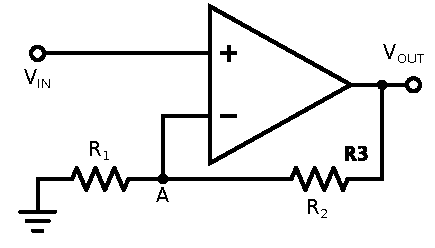
\includegraphics[width=.65\textwidth]{ccninv.pdf}
			\label{fig:ccninv}
			\caption{Amplificatore non invertente}
			
		\end{minipage}
\end{figure}

Il primo circuito da noi analizzato consiste in un amplificatore invertente accoppiato DC.
Lo schema è riportato in Fig.(\ref{fig:ccinv}).
Come vediamo, il nostro amplificatore operazionale è collegato con un circuito di \textbf{feedback} \textbf{negativo} (ovvero viene portato un po' del segnale in output all'ingresso invertente).
Così facendo possiamo avere un controllo sul segnale in uscita che altrimenti sarebbe, per come è costruito l'op-amp, $\pm V$ (avendo un guadagno di $10^6$).

Se consideriamo il nostro amplificatore operazionale ideale, abbiamo che $\Delta V_{12}=0$ (prima condizione di idealità).
Il punto $A$ sarà un ground virtuale.
Possiamo dunque imporre $I_1=\frac{V_{in}-V_A}{R_1}=\frac{V_{in}}{R_1}$.
Inoltre $I_2=\frac{V_A-V_{out}}{R_2}=\frac{-V_{out}}{R_2}$.
Sfruttando la seconda condizione di idealità, $\Delta I_{12}=0$, otteniamo $V_{out}=-\frac{R_2}{R_1} V_{in}$.
Il guadagno del nostro circuito amplificatore sarà dunque:

$$G=-\frac{R_2}{R_1}$$

Esso è negativo in quanto sfasato rispetto al segnale in ingresso di $\pi$.
La richiesta fatta era di ottenere un guadagno di circa -10.
Abbiamo dunque scelto di usare $R_1=(1001.6\pm0.3)\Omega$ e $R_2=(9987.1\pm0.3)\Omega$.
Il circuito è stato alimentato con un segnale in input sinusoidale alla frequenza di 1kHz.
Per valori picco-picco maggiori di $3V$ abbiamo notato l'ormai classico effetto di clapping del segnale, in quanto la tensione in output raggiungeva il valore massimo fornito dalla polarizzazione DC dell'op-amp. 

Ne abbiamo inoltre analizzato l'andamento al variare della frequenza.
Come già accaduto per l'amplificatore alle differenze, abbiamo notato che a frequenze elevato il guadagno diminuiva considerevolmente, con anche uno sfasamento rilevante dei segnali.
In Fig.(??) è riportato un grafico del guadagno in funzione della frequenza. 

$$Grafico??$$

$$Se abbiamo i dati$$


Crediamo che il motivo di tale smorzamento del segnale sia la presenza dei transistor e delle capacità nell'amplificatore operazionale.


Successivamente abbiamo montato l'amplificatore non invertende come mostrato in Fig.(\ref{fig:ccninv}). Con gli stessi ragionamenti fatti sopra, possiamo calcolare il guadagno di tale circuito: $V_A=V_{in}=V_{out}\frac{R_1}{R_2+R_1} \Rightarrow V_{out}=(1+\frac{R_2}{R_1})$. Il guadagno, positivo in questo caso, risulta essere: 

$$G=1+\frac{R_2}{R_1}$$

Anche per questo circuito abbiamo analizzato la risposta in frequenza.
Il risultato ottenuto è identico a quello per il circuito precedentemente analizzato e dunque abbiamo deciso di non riportare un grafico.

\begin{wrapfigure}[12]{r}[0pt]{65mm}
	\caption{Circuito sommatore}
	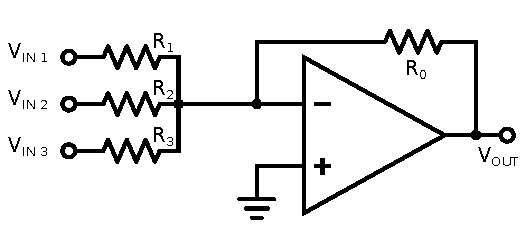
\includegraphics[width=65mm]{ccsum.pdf}
	\label{fig:ccsum}
\end{wrapfigure}

\section{Sommatore}

Il circuito riportato in Fig.(\ref{}) è lo schema di un sommatore.
Tale circuito permette la somma di più segnali in input e risulta particolarmente comodo nel caso, ad esempio, della necessità di trasformare un numero digitale (bit) in numero analogico.
Analizziamo il circuito sempre assumendo un op-amp ideale.
Anche in questo caso $V_A$ sarà un ground virtuale.
Possiamo dunque imporre la seguente condizione: $\frac{V_1}{R_1}+\frac{V_2}{R_2}+\frac{V_3}{R_3}=\frac{-V_{out}}{R_0}$.
Dunque, se $R_0=R_1=R_2=R_3$ segue immediamtamente che $V_{out}=V_1+V_2+V_3$.
Ne abbiamo verificato il funzionamento utilizzando diversi segnali in input (tra cui onde quadre, segnali DC, cardiodi (???), ecc.).
Nelle seguenti figure sono riportati i segnali visualizzati a schermo sull'oscilloscopio.

$$grafici$$

Come vediamo il circuito si comporta da sommatore. I valori di resistenza utilizzate sono stati $R_0=(10.01\pm0.02)\si{\kilo\ohm}$, $R_1=(9.95\pm0.01)\si{\kilo\ohm}$, $R_2=(10.02\pm 0.01)\si{\kilo\ohm}$ e $R_3=(9.97\pm0.01)\si{\kilo\ohm}$.

\begin{wrapfigure}[12]{r}[0pt]{65mm}
	\caption{Circuito sommatore}
	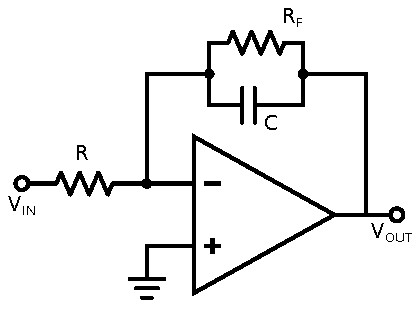
\includegraphics[width=65mm]{ccint.pdf}
	\label{fig:ccsum}
\end{wrapfigure}

\section{Integratore}

In questa parte dell'esperienza utilizzeremo un cazzo di op-amp per costruire un circuito integratore. Lo schema è riportato in Fig.(\ref{}). Analizziamolo assumendo che $R_f=\infty$\footnote{Senza tale approssimazione risulta particolarmente complicata la trattazione del circuito.}. È semplice ricavare $I=C\frac{d(V_A-V_{out})}{dt}$ da cui $V_{in}=-RC\frac{V_{out}}{dt}$. Non siamo matematici ma la seguente relazione è triviale:

$$V_{out}=-\frac{1}{RC} \int V_{in}dt +costante$$

I valori di resistenze e capacità utilizzate sono $R=(99.2 \pm 0.1)\si{\kilo\ohm}$, $R_f=(2.247 \pm 0.001)\si{\mega\ohm}$ e $C=(0.097 \pm 0.002) \si{\micro\farad}$. 

Poiche il condensatore, come sappiamo, taglia i segnali continui, dobbiamo preoccuparci di calcolare la frequenza di taglio. Assumendo trascurabile il contributo dato da $R_f$ e dalla resistenza interna dell'oscilloscopio (entrambe molto grandi, dell'ordine del $\si{\mega\ohm}$), la frequenza di taglio approssimativamente è stimabile da $f\simeq \frac{1}{2\pi C R_1}$. Inserendo i valori numerici otteniamo $f \simeq 15 \si{\hertz}$. Abbiamo dunque deciso di utilizzare dei segnali in ingresso a frequenza di \SI{10}{\hertz}. Abbiamo tuttavia provato anche per frequenze di \SI{1}{\kilo\hertz}. I risultati sono esposti nei seguenti grafici.

\begin{wrapfigure}[12]{r}[0pt]{65mm}
	\caption{Circuito sommatore}
	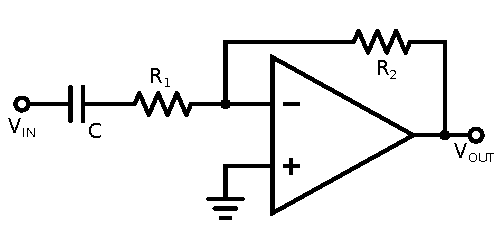
\includegraphics[width=65mm]{ccder.pdf}
	\label{fig:ccsum}
\end{wrapfigure}

\section{Derivatore}